

%%%CONTEMPORARY%%%
\documentclass[unnumsec,webpdf,contemporary,large]{oup-authoring-template}%


% line numbers
%\usepackage[mathlines, switch]{lineno}
%\usepackage[right]{lineno}
\usepackage{svg}
\theoremstyle{thmstyleone}%
\newtheorem{theorem}{Theorem}%  meant for continuous numbers
%%\newtheorem{theorem}{Theorem}[section]% meant for sectionwise numbers
%% optional argument [theorem] produces theorem numbering sequence instead of independent numbers for Proposition
\newtheorem{proposition}[theorem]{Proposition}%
%%\newtheorem{proposition}{Proposition}% to get separate numbers for theorem and proposition etc.
\theoremstyle{thmstyletwo}%
\newtheorem{example}{Example}%
\newtheorem{remark}{Remark}%
\theoremstyle{thmstylethree}%
\newtheorem{definition}{Definition}

\begin{document}

\journaltitle{701: Computational Genomics}
\DOI{May 16, 2024}
\copyrightyear{2024}
\pubyear{2014}
\access{}
\appnotes{Paper}

\firstpage{1}

%\subtitle{Subject Section}

\title[Salmon: Combining Inference Modes]{Salmon: Combining Inference Modes}

\author[1]{Nathalie Bonin}
\author[1]{Annie Dai}
\author[1]{Emma Shroyer}

% \authormark{Author Name et al.}

\address[1]{\orgdiv{Computer Science Department}, \orgname{University of Maryland}, \orgaddress{\state{Maryland}, \country{USA}}}

% \corresp[$\ast$]{Corresponding author. \href{email:email-id.com}{email-id.com}}




\abstract{Salmon provides a fast and accurate way to estimate transcript abundance. 
This method uses a dual-phase inference algorithm and takes into account fragment biases for transcript verification. 
However, there are some areas where Salmon could improve. 
The inference algorithms used—EM and VBEM—are only point estimates and cannot be checked if there is 
no ground truth available. 
Furthermore, the choice of prior when using the VBEM algorithm can affect the accuracy of the results. 
In this work, we test how averaging the inference model predictions affect the accuracy of the inference estimation 
during Salmon’s 
offline phase. }
\keywords{Salmon, Tuna, Onefish, Twofish, Redfish, Bluefish}


\maketitle
\section{Introduction}

A key characteristic of many newly-formed eukaryotic RNA sequences is the inclusion of non-coding and coding regions, 
which are often referred to as introns and exons. Prior to translation, transcript maturation must occur via splicing, 
a process that revolves around the displacement of introns from the mRNA sequence. However, depending on environmental 
conditions and sequence variations, some exons are often removed from the mRNA as well, eventually resulting in the creation of 
a different protein isoform. Unfortunately, the many factors related to alternative splicing are still poorly understood for most 
eukaryotic proteins, hence the reasoning behind the continuation of transcriptome projects.\\

One essential facet to transcriptomics is the sequencing techniques used to generate transcript fragments for data analysis. 
Prior approaches to transcriptome quantification involved the use of microarrays, which has important limitations such as relatively high 
risks of cross-hybridization, low range of detection, and complicated normalization methods for differential expression analysis 
\cite{Wang_Gerstein_Snyder_2009}. 
RNA-Seq, on the other hand, does not face such limitations and retains microarrays’ advantage over classical sequencing such as 
high-throughput capabilities and the use of inexpensive technology. It has been revolutionary in furthering the field of transcriptomics,
specifically with regards to eukaryotic cell transcriptomes. In particular, recent RNA-seq experiments yielded meaningful results in 
quantifying expression difference across different tissues \cite{Glinos_et_al._2022}, distinguishing host-pathogen interactions 
\cite{Pisu_Huang_Grenier_Russell_2020}, 
and identifying the effect of structural variants on splicing regulators \cite{Pascal_et_al._2023}. \\

Equally important to transcriptomics is abundance quantification. Estimations can be done through an alignment to a 
reference transcriptome sequence; nevertheless, a constant struggle with quantifying eukaryotic samples is to map read 
fragments back to the original transcript as opposed to the original gene. Although the detection of protein family abundances 
can be useful on its own, oftentimes researchers are more so interested in transcript abundances. Since isoforms of the same 
protein will retain common exons, identifying the source of each read is a tedious process that requires 
complex statistical methods.\\

In the past, Salmon was developed to address this particular issue. Given a known transcript and a set of sequenced fragments, 
it quantifies the relative abundance of each transcript in the sample using a dual-phase inference procedure. 
Salmon improves accuracy compared to other models, because it takes into account sample-specific biases to improve accuracy. 
When these biases are not accounted for, calculations like the false discovery rate cannot be controlled for. 
Using multiple inference steps, Salmon improves its abundance estimates using either the VBEM or EM inference algorithms. 
However, both methods have drawbacks. Both algorithms return point estimates of abundances, and we are uncertain about the returned 
estimates without ground truth. Further, the choice of  Bayesian priors used in the VBEM algorithm also has considerations. 
A small prior leads to sparser results than EM. However, a larger prior may result in more estimated non-zero abundance than EM. 
Prior simulated tests \cite{noauthor_salmon_nodate} show that VBEM with a small prior can lead to more accurate estimates. However, 
there has been much research into improving the results of these algorithms such as model averaging \cite{hoeting_bayesian_1999}. 
Given the trade offs of the two algorithms, we sought to know if the averaged prediction for EM and VBEM inference is better than 
one algorithm or another. Further, if this ensemble estimate is better, could it be improved by varying the Bayesian priors.
We have found that the average of these outputs did not result in conclusive results. \\

We saw that using the average is very similar to EM when used with a higher prior and more similar to the VBEM output when used with 
a higher prior. In light of these results we have also included a section on future work. 

\section{Methods}
\subsection{Combining the traditional EM algorithm with the VBEM algorithm}
Since we are only interested in optimizing abundance estimation in the offline phase, we opted to directly change Salmon v1.10.3’s 
source code. We introduce a new flag, $\mathtt{--useBoth}$, which forces the program to run the offline phase twice: 
once with the traditional EM algorithm and once with the VBEM algorithm. 
The program then computes the average of the two different estimates for the $\pmb{\alpha}$ vector before computing its final 
prediction for $\pmb{\eta}$.

\subsection{Running the new implementation on the polyester dataset}
The commands used for the quantification of each sample using EM, VBEM, or both inference strategies, are provided in Fig \ref{code}.
\begin{figure*}[!t]%
    \centering
    {        
        \begin{verbatim}
        salmon quant -i human_index -l IU -1 sample_1.fa.gz -2 sample_2.fa.gz -p 6 --gcBias --useEM \
            --validateMappings -o sample
        salmon quant -i human_index -l IU -1 sample_1.fa.gz -2 sample_2.fa.gz -p 6 --gcBias --vbPrior \
            1e{from -5 to 1} --validateMappings -o sample
        salmon quant -i human_index -l IU -1 sample_1.fa.gz -2 sample_2.fa.gz -p 6 --gcBias --useBoth \
            --vbPrior 1e{from -5 to 1} --validateMappings -o sample
    \end{verbatim}
    }
    \caption{Commands used for the quantification of each sample using EM, VBEM, or both inference strategies, respectively.}
    \label{code}
\end{figure*}

Quantification was run on the 24 samples through a slurm batch script. 
For each run, 5GB of memory was allocated on the CBCB’s Nexus partition. 
In total, every sample had 15 runs, each with different specifications for the inference method (1 EM, 7 VBEM, and 7 combo) 
and the prior value if applicable ($10^{-5}$ to $10^1$).  All other parameters were kept the same among the 360 total runs: 
\begin{enumerate}
    \item We kept the selective alignment feature on for this experiment. This strategy is currently the default for the pipeline, 
    and it allows Salmon to adopt a more sensitive approach during quasi-mapping.
    \item In recent versions of Salmon, the library type can be automatically detected. Nevertheless, we elected to 
    specify the library type for all the runs.
    \item The $\mathtt{–gcBias}$ flag was passed to the pipeline as well, which allows Salmon to identify and  remedy for 
    GC biases. This extra step is essential for the analysis of our synthetic data since they were simulated from an already 
    existing GC bias profile \cite{love_swimming_2018}.
    
\end{enumerate}

\section{Evaluation}
\[
    \mathrm{ARD}_i = \begin{cases}
        0 &\quad\text{if}\quad x_i = y_i = 0\\
        \dfrac{\left| x_i-y_i \right| }{x_i-y_i} &\quad\text{otherwise}\quad
    \end{cases}
\]

\[
    \mathrm{MARD} = \frac{1}{M} \sum^{M}_{i = 1}\mathrm{ARD}_i
\]
\subsection{Spearman Correlation}
\[
    \rho = 1 - \dfrac{6 \sum{d^2_i}}{n(n^2-1)}
\]
\subsection{Mann–Whitney U Test}
\subsection{Datasets}
We used synthetic datasets in the same form as \cite{patro_salmon_2017}. 
We generated our synthetic data using polyester 1.16.0 and alpine version 1.6.0. 
[citation] There was ground truth available for this dataset. We additionally used real human datasets. 
We used a dataset consisting of NK cells, T cells, and tumor from matched soft tissue sarcoma and peripheral 
blood collected from soft tissue sarcomas patients who had undergone surgery. 
[citation] We also utilized the human transcriptome reference: Homo sapiens GRCh38 cDNA sequence. 
These were gene models built from alignments of the human proteome and alignments of human cDNAs. [citation]

\section{Results}
We encountered different results depending on the prior selected. Overall, we can separate the outcome of combining both inference algorithms into two categories. The first of such categories includes runs with a prior between $10^{-5}$ and $10^1$, inclusive. As shown in figures \ref{speartable} and \ref{mardtable}, both the $\mathrm{MARD}$ values and the Spearman correlation values are lower for estimates inferred from VBEM than for estimates inferred from both methods (Mann-Whitney U test, $P\leq 1.436 \cdot  10^{-7}$ for MARD, $P < 6.202\cdot 10^{-14}$ for Spearman). However, MARD values tended to be similar between estimates inferred from EM and estimates inferred from both methods (Mann-Whitney U test, $P\geq 0.4803$), whereas the Spearman correlation values were slightly higher for EM (Mann-Whitney U test, $P\leq 0.03941$). Because the MARD metrics are negatively impacted by false discovery rates \cite{patro_salmon_2017}, we hypothesize that the results gathered from running both inference algorithms is affected by EM’s tendency to collect more non-zero abundances than VBEM at low prior values. 

This can also be concluded from the analysis of our second category, which includes runs with a prior of 1 or 10. Unlike with the first category, the $\mathrm{MARD}$ and the Spearman correlation values are strikingly lower for the estimates inferred from EM (Mann-Whitney U test, $P < 6.202\cdot 10^{-14}$ for $\mathrm{MARD}$, $P < 6.202\cdot 10^{-14}$ for Spearman), whereas the difference in MARD between VBEM and the combination of both methods was insignificant for runs with a prior of 1 (Mann-Whitney U test, $P = 0.8944$). The difference between the Spearman correlation values and between the MARD values for runs with a prior of 10 was still significant (Mann-Whitney U test, $P = 5.675 \cdot 10^{-11}$ for $\mathrm{MARD}$, $P < 6.202\cdot 10^{-14}$ for Spearman). We predict that this would suggest that for high prior values, the negative impact from false discovery rates by the VBEM algorithm is offsetted by the more accurate abundance estimates from the EM algorithm. 
\begin{table*}[t]
    \caption{Spearman correlation table for first four samples and their subsamples.
    \label{speartable}}
    \tabcolsep=0pt%%
    \begin{tabular*}{\textwidth}{@{\extracolsep{\fill}}lcccccc@{\extracolsep{\fill}}}
    \toprule
    \begin{tabular}{lrrrrrrrr}
        \textbf{} &
          \multicolumn{1}{l}{Sample $1_{01}$} &
          \multicolumn{1}{l}{Sample $1_{02}$} &
          \multicolumn{1}{l}{Sample $2_{01}$} &
          \multicolumn{1}{l}{Sample $2_{02}$} &
          \multicolumn{1}{l}{Sample $3_{01}$} &
          \multicolumn{1}{l}{Sample $3_{02}$} &
          \multicolumn{1}{l}{Sample $4_{01}$} &
          \multicolumn{1}{l}{Sample $4_{02}$} \\
        EM           & 0.932 & 0.932 & 0.933 & 0.932 & 0.937 & 0.936 & 0.934 & 0.933 \\
        both - $10^{-5}$ & 0.933 & 0.933 & 0.934 & 0.933 & 0.939 & 0.938 & 0.935 & 0.934 \\
        VBEM - $10^{-5}$ & 0.952 & 0.951 & 0.953 & 0.951 & 0.957 & 0.956 & 0.954 & 0.952 \\
        both - $10^{-4}$ & 0.933 & 0.933 & 0.934 & 0.933 & 0.939 & 0.938 & 0.935 & 0.934 \\
        VBEM - $10^{-4}$ & 0.952 & 0.951 & 0.953 & 0.951 & 0.957 & 0.956 & 0.954 & 0.952 \\
        both - $10^{-3}$ & 0.933 & 0.933 & 0.934 & 0.933 & 0.939 & 0.938 & 0.935 & 0.934 \\
        VBEM - $10^{-3}$ & 0.952 & 0.951 & 0.953 & 0.951 & 0.957 & 0.956 & 0.954 & 0.952 \\
        both - $10^{-2}$ & 0.933 & 0.933 & 0.934 & 0.933 & 0.939 & 0.938 & 0.935 & 0.934 \\
        VBEM - $10^{-2}$ & 0.952 & 0.951 & 0.953 & 0.952 & 0.957 & 0.956 & 0.954 & 0.952 \\
        both - $10^{-1}$ & 0.933 & 0.933 & 0.934 & 0.933 & 0.939 & 0.937 & 0.935 & 0.934 \\
        VBEM - $10^{-1}$ & 0.951 & 0.950 & 0.953 & 0.951 & 0.957 & 0.955 & 0.954 & 0.951 \\
        both - $10^{0}$  & 0.755 & 0.754 & 0.755 & 0.754 & 0.755 & 0.755 & 0.755 & 0.754 \\
        VBEM - $10^{0}$  & 0.751 & 0.751 & 0.751 & 0.751 & 0.752 & 0.752 & 0.751 & 0.751 \\
        both - $10^{1}$  & 0.736 & 0.735 & 0.736 & 0.736 & 0.738 & 0.737 & 0.736 & 0.736 \\
        VBEM - $10^{1}$  & 0.715 & 0.715 & 0.715 & 0.716 & 0.717 & 0.717 & 0.715 & 0.715 \\
        \botrule    
    \end{tabular}
    
    \end{tabular*}
    \end{table*}
\section{Discussion}

In the current timeframe, we were unable to expand on our project but in future work, we would like to expand upon ways to best combine the results of the EM and VBEM algorithms. Currently we are only taking the mean of the two results. However, we would also like to experiment with the weighted average or the Bayesian model average of these two algorithms also taking into account various prior sizes. We hypothesize that this would further improve Salmon’s results. \cite{doi:10.1177/2515245919898657}


We would also like to verify the time it takes to run our combined approach. We would like to verify that running this approach will not greatly impact the runtime of Salmon. While we expect the runtime to increase; however, we would like to verify that it is not detrimental to the use of Salmon. 

In future work, it will be beneficial to get a measure of uncertainty when running our trials. We were unable to run this during our initial experiments. However, we would like to know if there is a level of uncertainty with our results when we use the average of the EM and VBEM algorithms. We would like to know if this uncertainty increases or decreases, and if so, is the change in uncertainty significantly. Salmon already supports this analysis through the use of a flag. 

\section{Future Work}
In our results we saw that using the average of both VBEM and EM is very similar to EM 
when used with a lower prior and more similar to the VBEM output when used with a higher prior. 
We have hypothesized this is because we were taking the average even when one of the results was a 
zero. In future work, we would like to prioritize zero abundances over non-zero abundances. 
Instead of taking the average between value and zero, we want to record the value as zero. 
If neither result is a zero, we wish to take the average of those values. 
We believe this could improve our estimates. 

In the current timeframe, we were unable to expand on our project, but in future work, 
we would like to expand upon ways to best combine the results of the EM and VBEM algorithms. 
Currently, our code is only taking the mean of the two results. 
However, we would also like to experiment with the weighted average or the Bayesian model average 
of these two algorithms also taking into account various prior sizes. 
We hypothesize that this would further improve Salmon’s results \cite{patro_salmon_2017}. 
Additionally, we also would like to test our approach on real life data. 
Although we picked out a dataset consisting of sequencing reads from NK cells, T cells, 
and tumor collected from matched soft tissue sarcoma and peripheral blood \cite{judge_transcriptome_2022}, we were pressed 
for time and resources, and therefore we had to abandon this portion of our project.

We would also like to verify the time it takes to run our combined approach. 
It would be beneficial to run multiple trials to gain an idea of the time it takes to run 
Salmon using our solution. We would like to verify that running this approach will not greatly 
impact the runtime of Salmon. The runtime is expected to increase, since we are running both the 
EM and VBEM algorithms. However, we would like to verify that it is not detrimental to the use 
of Salmon. 

In future work, it would be useful to measure the uncertainty of our trials. 
We were unable to run this during our initial experiments. However, we would like to know if there 
is a level of uncertainty with our results when we use the average of the EM and VBEM algorithms. 
We would like to know if this uncertainty increases or decreases, and if so, whether the change in 
uncertainty is significant. Salmon already supports this analysis through the use of a flag. 




\bibliographystyle{plain}
\bibliography{reference}
\section{Supplementary}
\begin{table*}[t]
  \caption{Spearman correlation table for first four samples and their subsamples.}
  \label{speartable}
  \tabcolsep=0pt%%
  \begin{tabular*}{\textwidth}{@{\extracolsep{\fill}}lrrrrrrrr@{\extracolsep{\fill}}}
  \toprule%
  \textbf{} &
  \multicolumn{1}{l}{Sample $1_{01}$} &
  \multicolumn{1}{l}{Sample $1_{02}$} &
  \multicolumn{1}{l}{Sample $2_{01}$} &
  \multicolumn{1}{l}{Sample $2_{02}$} &
  \multicolumn{1}{l}{Sample $3_{01}$} &
  \multicolumn{1}{l}{Sample $3_{02}$} &
  \multicolumn{1}{l}{Sample $4_{01}$} &
  \multicolumn{1}{l}{Sample $4_{02}$} \\
EM           & 0.932 & 0.932 & 0.933 & 0.932 & 0.937 & 0.936 & 0.934 & 0.933 \\
both - $10^{-5}$ & 0.933 & 0.933 & 0.934 & 0.933 & 0.939 & 0.938 & 0.935 & 0.934 \\
VBEM - $10^{-5}$ & 0.952 & 0.951 & 0.953 & 0.951 & 0.957 & 0.956 & 0.954 & 0.952 \\
both - $10^{-4}$ & 0.933 & 0.933 & 0.934 & 0.933 & 0.939 & 0.938 & 0.935 & 0.934 \\
VBEM - $10^{-4}$ & 0.952 & 0.951 & 0.953 & 0.951 & 0.957 & 0.956 & 0.954 & 0.952 \\
both - $10^{-3}$ & 0.933 & 0.933 & 0.934 & 0.933 & 0.939 & 0.938 & 0.935 & 0.934 \\
VBEM - $10^{-3}$ & 0.952 & 0.951 & 0.953 & 0.951 & 0.957 & 0.956 & 0.954 & 0.952 \\
both - $10^{-2}$ & 0.933 & 0.933 & 0.934 & 0.933 & 0.939 & 0.938 & 0.935 & 0.934 \\
VBEM - $10^{-2}$ & 0.952 & 0.951 & 0.953 & 0.952 & 0.957 & 0.956 & 0.954 & 0.952 \\
both - $10^{-1}$ & 0.933 & 0.933 & 0.934 & 0.933 & 0.939 & 0.937 & 0.935 & 0.934 \\
VBEM - $10^{-1}$ & 0.951 & 0.950 & 0.953 & 0.951 & 0.957 & 0.955 & 0.954 & 0.951 \\
both - $10^{0}$  & 0.755 & 0.754 & 0.755 & 0.754 & 0.755 & 0.755 & 0.755 & 0.754 \\
VBEM - $10^{0}$  & 0.751 & 0.751 & 0.751 & 0.751 & 0.752 & 0.752 & 0.751 & 0.751 \\
both - $10^{1}$  & 0.736 & 0.735 & 0.736 & 0.736 & 0.738 & 0.737 & 0.736 & 0.736 \\
VBEM - $10^{1}$  & 0.715 & 0.715 & 0.715 & 0.716 & 0.717 & 0.717 & 0.715 & 0.715 \\
  \botrule
  \end{tabular*}
  % \begin{tablenotes}%
  % \item Note: This is an example of table footnote this is an example of table footnote this is an example of table footnote this is an example of~table footnote this is an example of table footnote
  % \item[$^{1}$] Example for a first table footnote.
  % \item[$^{2}$] Example for a second table footnote.\vspace*{6pt}
  % \end{tablenotes}
  \end{table*}

  

  \begin{table*}[t]
    \caption{MARD table for first four samples and their subsamples.}
    \label{mardtable}
    \tabcolsep=0pt%%
    \begin{tabular*}{\textwidth}{@{\extracolsep{\fill}}lrrrrrrrr@{\extracolsep{\fill}}}
    \toprule%
    \textbf{} &
    \multicolumn{1}{l}{Sample $1_{01}$} &
    \multicolumn{1}{l}{Sample $1_{02}$} &
    \multicolumn{1}{l}{Sample $2_{01}$} &
    \multicolumn{1}{l}{Sample $2_{02}$} &
    \multicolumn{1}{l}{Sample $3_{01}$} &
    \multicolumn{1}{l}{Sample $3_{02}$} &
    \multicolumn{1}{l}{Sample $4_{01}$} &
    \multicolumn{1}{l}{Sample $4_{02}$} \\
  EM           & 0.284 & 0.285 & 0.273 & 0.276 & 0.243 & 0.245 & 0.277 & 0.278 \\
  both - $10^{-5}$ & 0.287 & 0.287 & 0.275 & 0.278 & 0.245 & 0.247 & 0.279 & 0.280 \\
  VBEM - $10^{-5}$ & 0.241 & 0.243 & 0.229 & 0.232 & 0.199 & 0.201 & 0.233 & 0.235 \\
  both - $10^{-4}$ & 0.287 & 0.287 & 0.275 & 0.278 & 0.245 & 0.247 & 0.279 & 0.280 \\
  VBEM - $10^{-4}$ & 0.241 & 0.243 & 0.229 & 0.232 & 0.199 & 0.201 & 0.233 & 0.235 \\
  both - $10^{-3}$ & 0.287 & 0.287 & 0.275 & 0.278 & 0.245 & 0.247 & 0.279 & 0.280 \\
  VBEM - $10^{-3}$ & 0.241 & 0.243 & 0.229 & 0.232 & 0.199 & 0.201 & 0.232 & 0.235 \\
  both - $10^{-2}$ & 0.287 & 0.287 & 0.275 & 0.278 & 0.244 & 0.247 & 0.279 & 0.280 \\
  VBEM - $10^{-2}$ & 0.241 & 0.243 & 0.229 & 0.232 & 0.198 & 0.201 & 0.232 & 0.235 \\
  both - $10^{-1}$ & 0.286 & 0.287 & 0.274 & 0.277 & 0.244 & 0.246 & 0.278 & 0.280 \\
  VBEM - $10^{-1}$ & 0.241 & 0.243 & 0.229 & 0.232 & 0.199 & 0.201 & 0.233 & 0.235 \\
  both - $10^0$  & 0.663 & 0.662 & 0.658 & 0.658 & 0.647 & 0.647 & 0.660 & 0.660 \\
  VBEM - $10^0$  & 0.662 & 0.662 & 0.658 & 0.658 & 0.647 & 0.647 & 0.660 & 0.659 \\
  both - $10^1$  & 0.663 & 0.663 & 0.660 & 0.659 & 0.651 & 0.650 & 0.662 & 0.660 \\
  VBEM - $10^1$  & 0.678 & 0.678 & 0.675 & 0.674 & 0.667 & 0.666 & 0.677 & 0.675

    \botrule
    \end{tabular*}
    % \begin{tablenotes}%
    % \item Note: This is an example of table footnote this is an example of table footnote this is an example of table footnote this is an example of~table footnote this is an example of table footnote
    % \item[$^{1}$] Example for a first table footnote.
    % \item[$^{2}$] Example for a second table footnote.\vspace*{6pt}
    % \end{tablenotes}
    \end{table*}
  
    

% \begin{figure*}[!t]%
%     \centering
%     {        
%         \begin{table}[]
%             \begin{tabular}{lrrrrrrrr}
%             \textbf{} &
%               \multicolumn{1}{l}{Sample $1_{01}$} &
%               \multicolumn{1}{l}{Sample $1_{02}$} &
%               \multicolumn{1}{l}{Sample $2_{01}$} &
%               \multicolumn{1}{l}{Sample $2_{02}$} &
%               \multicolumn{1}{l}{Sample $3_{01}$} &
%               \multicolumn{1}{l}{Sample $3_{02}$} &
%               \multicolumn{1}{l}{Sample $4_{01}$} &
%               \multicolumn{1}{l}{Sample $4_{02}$} \\
%             EM           & 0.284 & 0.285 & 0.273 & 0.276 & 0.243 & 0.245 & 0.277 & 0.278 \\
%             both - $10^{-5}$ & 0.287 & 0.287 & 0.275 & 0.278 & 0.245 & 0.247 & 0.279 & 0.280 \\
%             VBEM - $10^{-5}$ & 0.241 & 0.243 & 0.229 & 0.232 & 0.199 & 0.201 & 0.233 & 0.235 \\
%             both - $10^{-4}$ & 0.287 & 0.287 & 0.275 & 0.278 & 0.245 & 0.247 & 0.279 & 0.280 \\
%             VBEM - $10^{-4}$ & 0.241 & 0.243 & 0.229 & 0.232 & 0.199 & 0.201 & 0.233 & 0.235 \\
%             both - $10^{-3}$ & 0.287 & 0.287 & 0.275 & 0.278 & 0.245 & 0.247 & 0.279 & 0.280 \\
%             VBEM - $10^{-3}$ & 0.241 & 0.243 & 0.229 & 0.232 & 0.199 & 0.201 & 0.232 & 0.235 \\
%             both - $10^{-2}$ & 0.287 & 0.287 & 0.275 & 0.278 & 0.244 & 0.247 & 0.279 & 0.280 \\
%             VBEM - $10^{-2}$ & 0.241 & 0.243 & 0.229 & 0.232 & 0.198 & 0.201 & 0.232 & 0.235 \\
%             both - $10^{-1}$ & 0.286 & 0.287 & 0.274 & 0.277 & 0.244 & 0.246 & 0.278 & 0.280 \\
%             VBEM - $10^{-1}$ & 0.241 & 0.243 & 0.229 & 0.232 & 0.199 & 0.201 & 0.233 & 0.235 \\
%             both - $10^0$  & 0.663 & 0.662 & 0.658 & 0.658 & 0.647 & 0.647 & 0.660 & 0.660 \\
%             VBEM - $10^0$  & 0.662 & 0.662 & 0.658 & 0.658 & 0.647 & 0.647 & 0.660 & 0.659 \\
%             both - $10^1$  & 0.663 & 0.663 & 0.660 & 0.659 & 0.651 & 0.650 & 0.662 & 0.660 \\
%             VBEM - $10^1$  & 0.678 & 0.678 & 0.675 & 0.674 & 0.667 & 0.666 & 0.677 & 0.675
%             \end{tabular}
%             \end{table}

%     }
%     \caption{MARD table for first four samples and their subsamples.}
%     \label{mardtable}
% \end{figure*}


% \includesvg{"Min, Median, and Max MARD.svg"}
% \includesvg{"Min, Median, and Max Spearman Correlation.svg"}

\begin{figure*}[!t]%
\centering
{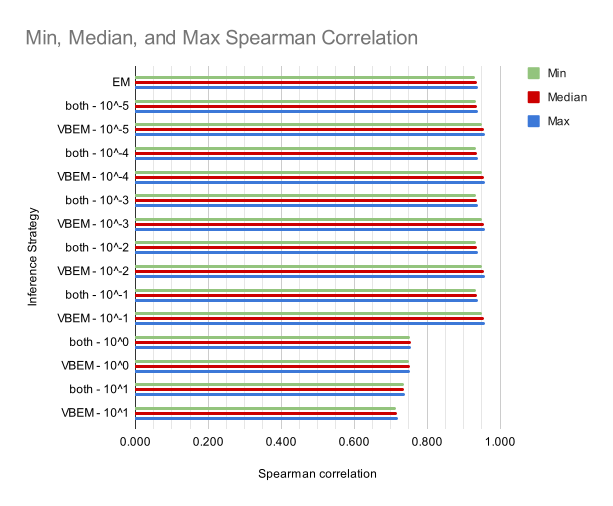
\includegraphics[width=\textwidth]{Min, Median, and Max Spearman Correlation.png}}
\caption{Min, Median, and Max Spearman Correlation}\label{spearfig}
\end{figure*}

\begin{figure*}[!t]%
  \centering
  {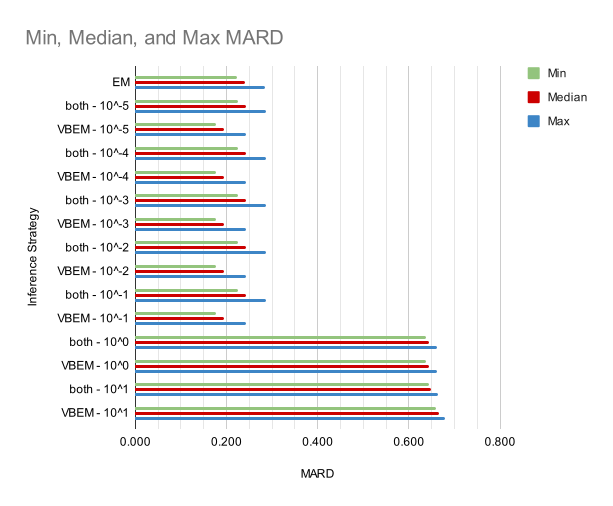
\includegraphics[width=\textwidth]{Min, Median, and Max MARD.png}}
  \caption{Min, Median, and Max MARD}\label{mardfig}
  \end{figure*}
% \begin{figure}
%     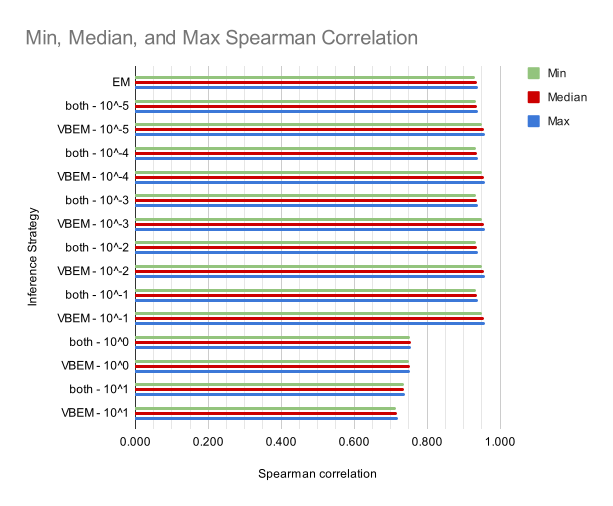
\includegraphics{Min, Median, and Max Spearman Correlation.png}
% \end{figure}
% \begin{figure}
% 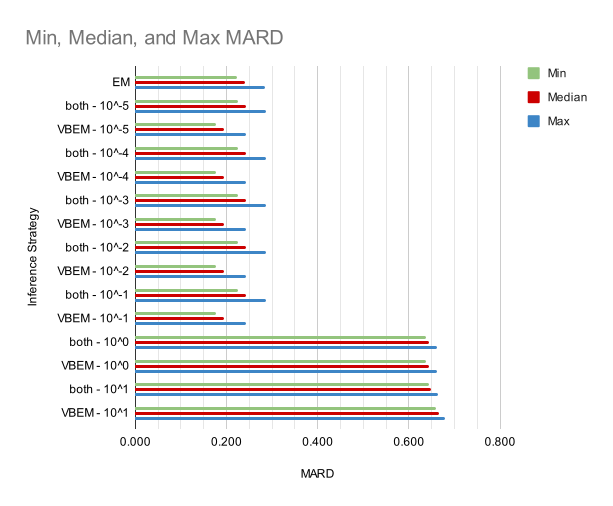
\includegraphics{Min, Median, and Max MARD.png}
% \end{figure}

\end{document}
